
\subsubsection{Use Case Diagrams}
Use case diagrams are a type of dynamic UML diagram that aim at illustrating the interactions between different actors (users or external systems) and the  system. They provide a high-level view of the ways the system collaborates with external entities, further details on each specific use case will be provided in the following sections of this document.

\begin{figure}[H]
	\centering
	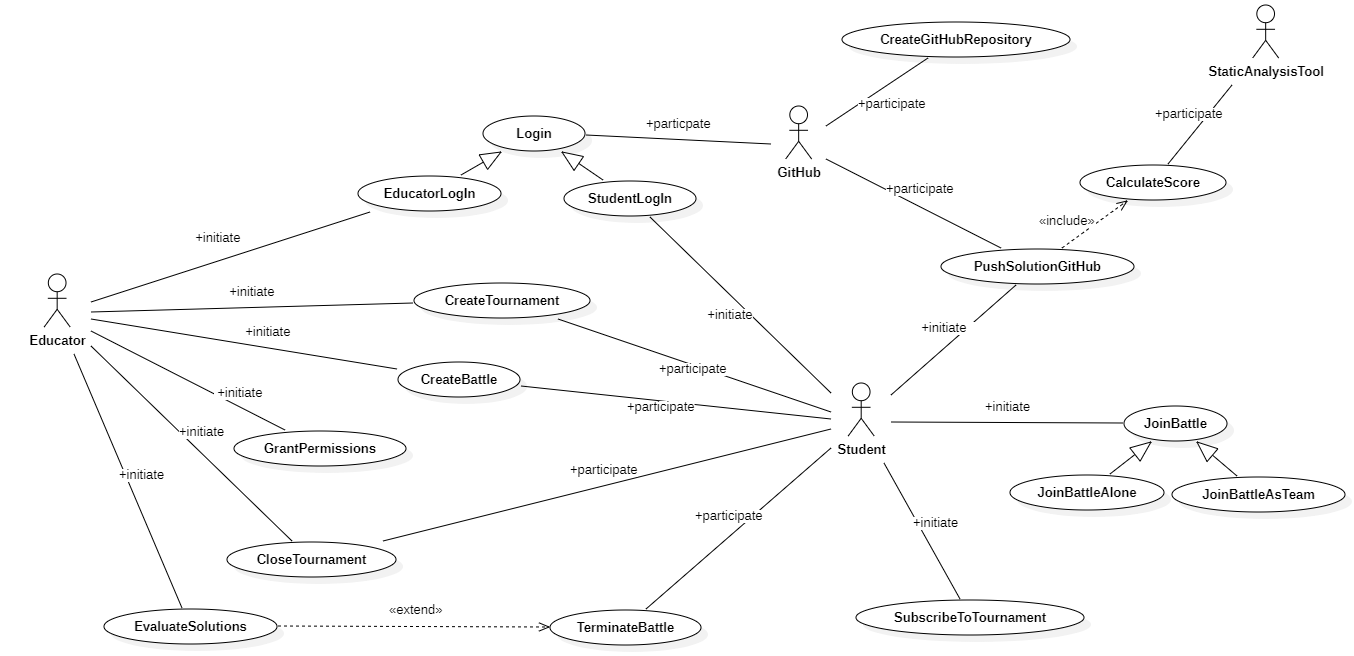
\includegraphics[width=16cm,keepaspectratio]{UseCaseDiagram1}
	
	\vspace{2cm}
	
	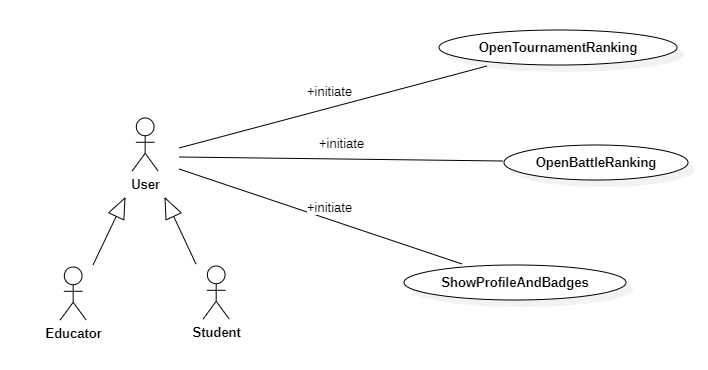
\includegraphics[width=10cm,keepaspectratio]{UseCaseDiagram2}
\end{figure}

The representation has been split into two different diagrams just for ease of reading. The Actors that are shown in the second diagram are the same as the ones in the diagram above. \\
Some of the use cases illustrated in the first diagram have relationships with other use cases. In particular:
\begin{itemize}
	\item \textbf{EvaluateSolutions} is an extension of \textbf{TerminateBattle}, meaning that EvaluateSolutions offers additional functionalities to the TerminateBattle use case when the consolidation stage is requested by the educator for his/her battle. It is not mandatory to have a consolidation stage for a battle, therefore the relationship is just an <<extend>> link.
	\item \textbf{PushSoluitonGitHub} includes \textbf{CalculateScore}. This is due to the fact that every time a student pushes a new code solution on GitHub, the process to compute the score to assign to that solution is triggered in the \app system. Therefore, PushSolutionGitHub leverages every time the use case CalculateScore and cannot be completed in a successful way without the included use case.
\end{itemize}
It is not the purpose of these diagrams to show the sequencing and temporal constraints that hold in the system between the various use cases. These analyses will be better shown through sequence and activity diagrams down the line of this document.